\documentclass[conference]{IEEEtran}
\IEEEoverridecommandlockouts
% The preceding line is only needed to identify funding in the first footnote. If that is unneeded, please comment it out.
\usepackage{cite}
\usepackage{amsmath,amssymb,amsfonts}
\usepackage{algorithmic}
\usepackage{graphicx}
\usepackage{textcomp}
\usepackage{xcolor}
\usepackage{booktabs}
\usepackage{url}
\usepackage{hyperref}

\hypersetup{
    colorlinks=true,
    linkcolor=blue,
    filecolor=magenta,      
    urlcolor=cyan,
    citecolor=blue
}

\def\BibTeX{{\rm B\kern-.05em{\sc i\kern-.025em b}\kern-.08em
    T\kern-.1667em\lower.7ex\hbox{E}\kern-.125emX}}

\begin{document}

\title{Wellsy: A Multi-Agent Jarvis-Class Desktop Operating Assistant with Dynamic Trust Tiers, Local Encrypted Memory, and Asynchronous Human-in-the-Loop Safeguards}

\author{\IEEEauthorblockN{Mokshith Nunna}
\IEEEauthorblockA{\textit{Department of Mechanical Engineering} \\
\textit{Amrita Vishwa Vidyapeetham}\\
Amritapuri, India \\
mokshithnunna31@gmail.com}
\and
\IEEEauthorblockN{Collaborators \& Research Team}
\IEEEauthorblockA{\textit{School of Computing \& Engineering} \\
\textit{Amrita Vishwa Vidyapeetham}\\
Amritapuri, India}
}

\maketitle

\begin{abstract}
Autonomous desktop operating assistants powered by Large Language Models (LLMs) present a paradigm shift in personal computing productivity. However, deploying multi-tool autonomous agents directly on host operating systems introduces critical vulnerabilities: destructive system modifications, privacy invasion via uncontrolled filesystem indexing, and high cognitive overhead caused by intrusive confirmation dialogs. In this paper, we introduce \textbf{Wellsy}, an open-source, Jarvis-class desktop operating intelligence framework that reconciles autonomous agency with robust safety and privacy guarantees. Wellsy is structured around four foundational pillars: (i) a \textbf{Three-Mode Architecture} providing seamless transitions between a futuristic holographic Web HUD, a non-blocking system tray daemon, and a high-efficiency command-line interface (CLI); (ii) a \textbf{Hierarchical Multi-Agent Graph} built on LangGraph that decomposes complex multi-domain user intents into five sandboxed sub-agents (Task, OS, Communications, Media, and Research); (iii) an \textbf{Asynchronous Human-in-the-Loop (HITL) Trust Tier Engine} that stratifies tool invocations into four granular risk tiers and non-blockingly halts execution only for dangerous actions; and (iv) a \textbf{Privacy-Preserving Episodic Memory} that computes zero-payload metadata delta snapshots across local workspaces, secured by AES-256 Fernet-encrypted SQLite storage. Comprehensive grey-box evaluation demonstrates that Wellsy achieves a 100\% interception rate on hazardous operations with zero false-positive interruptions on read-only queries, while sustaining sub-50\,ms supervisor routing latencies.
\end{abstract}

\begin{IEEEkeywords}
Autonomous Agents, Desktop Operating Intelligence, Human-in-the-Loop (HITL), Trust Tiers, LangGraph, AI Safety, Privacy-Preserving Computing.
\end{IEEEkeywords}

\section{Introduction}
Recent breakthroughs in foundational Large Language Models (LLMs) and communicative multi-agent frameworks \cite{vaswani2017attention, wu2023autogen, hong2023metagpt} have catalyzed interest in autonomous operating system (OS) assistants \cite{xie2024osworld, yang2023appagent}. Traditional graphical user interfaces (GUIs) and rigid command-line scripts require users to explicitly bridge domain boundaries---such as inspecting files, updating calendars, querying research papers, and scheduling background jobs. While conversational assistants have addressed high-level conceptual inquiries, deploying LLM agents capable of directly invoking native system tools and mutating the filesystem introduces severe security, privacy, and usability challenges \cite{greshake2023not, amodei2016concrete}.

Specifically, current desktop agent paradigms suffer from three fatal limitations:
\begin{enumerate}
    \item \textbf{Unchecked Autonomous Action Execution:} Existing frameworks often grant agents unconstrained execution privileges (e.g., executing arbitrary Bash/PowerShell commands or deleting directories). A single prompt injection or hallucinated instruction can permanently destroy local artifacts or leak sensitive credentials \cite{carlini2021extracting}.
    \item \textbf{Intrusive vs. Absent Confirmation Gates:} Existing safety mechanisms either prompt the user synchronously for every benign action---causing rapid human alarm fatigue---or execute completely unattended with zero safeguards.
    \item \textbf{Privacy Violations in Ambient Sensing:} Many local AI assistants continuously ingest full file contents and audio streams into unencrypted memory stores or external cloud endpoints, exposing user intellectual property and proprietary source code.
\end{enumerate}

To overcome these fundamental hurdles, we present \textbf{Wellsy}, a resilient, multi-agent desktop operating system designed for enterprise-grade safety, privacy, and continuous ambient interaction. 

\begin{figure*}[t]
\centering
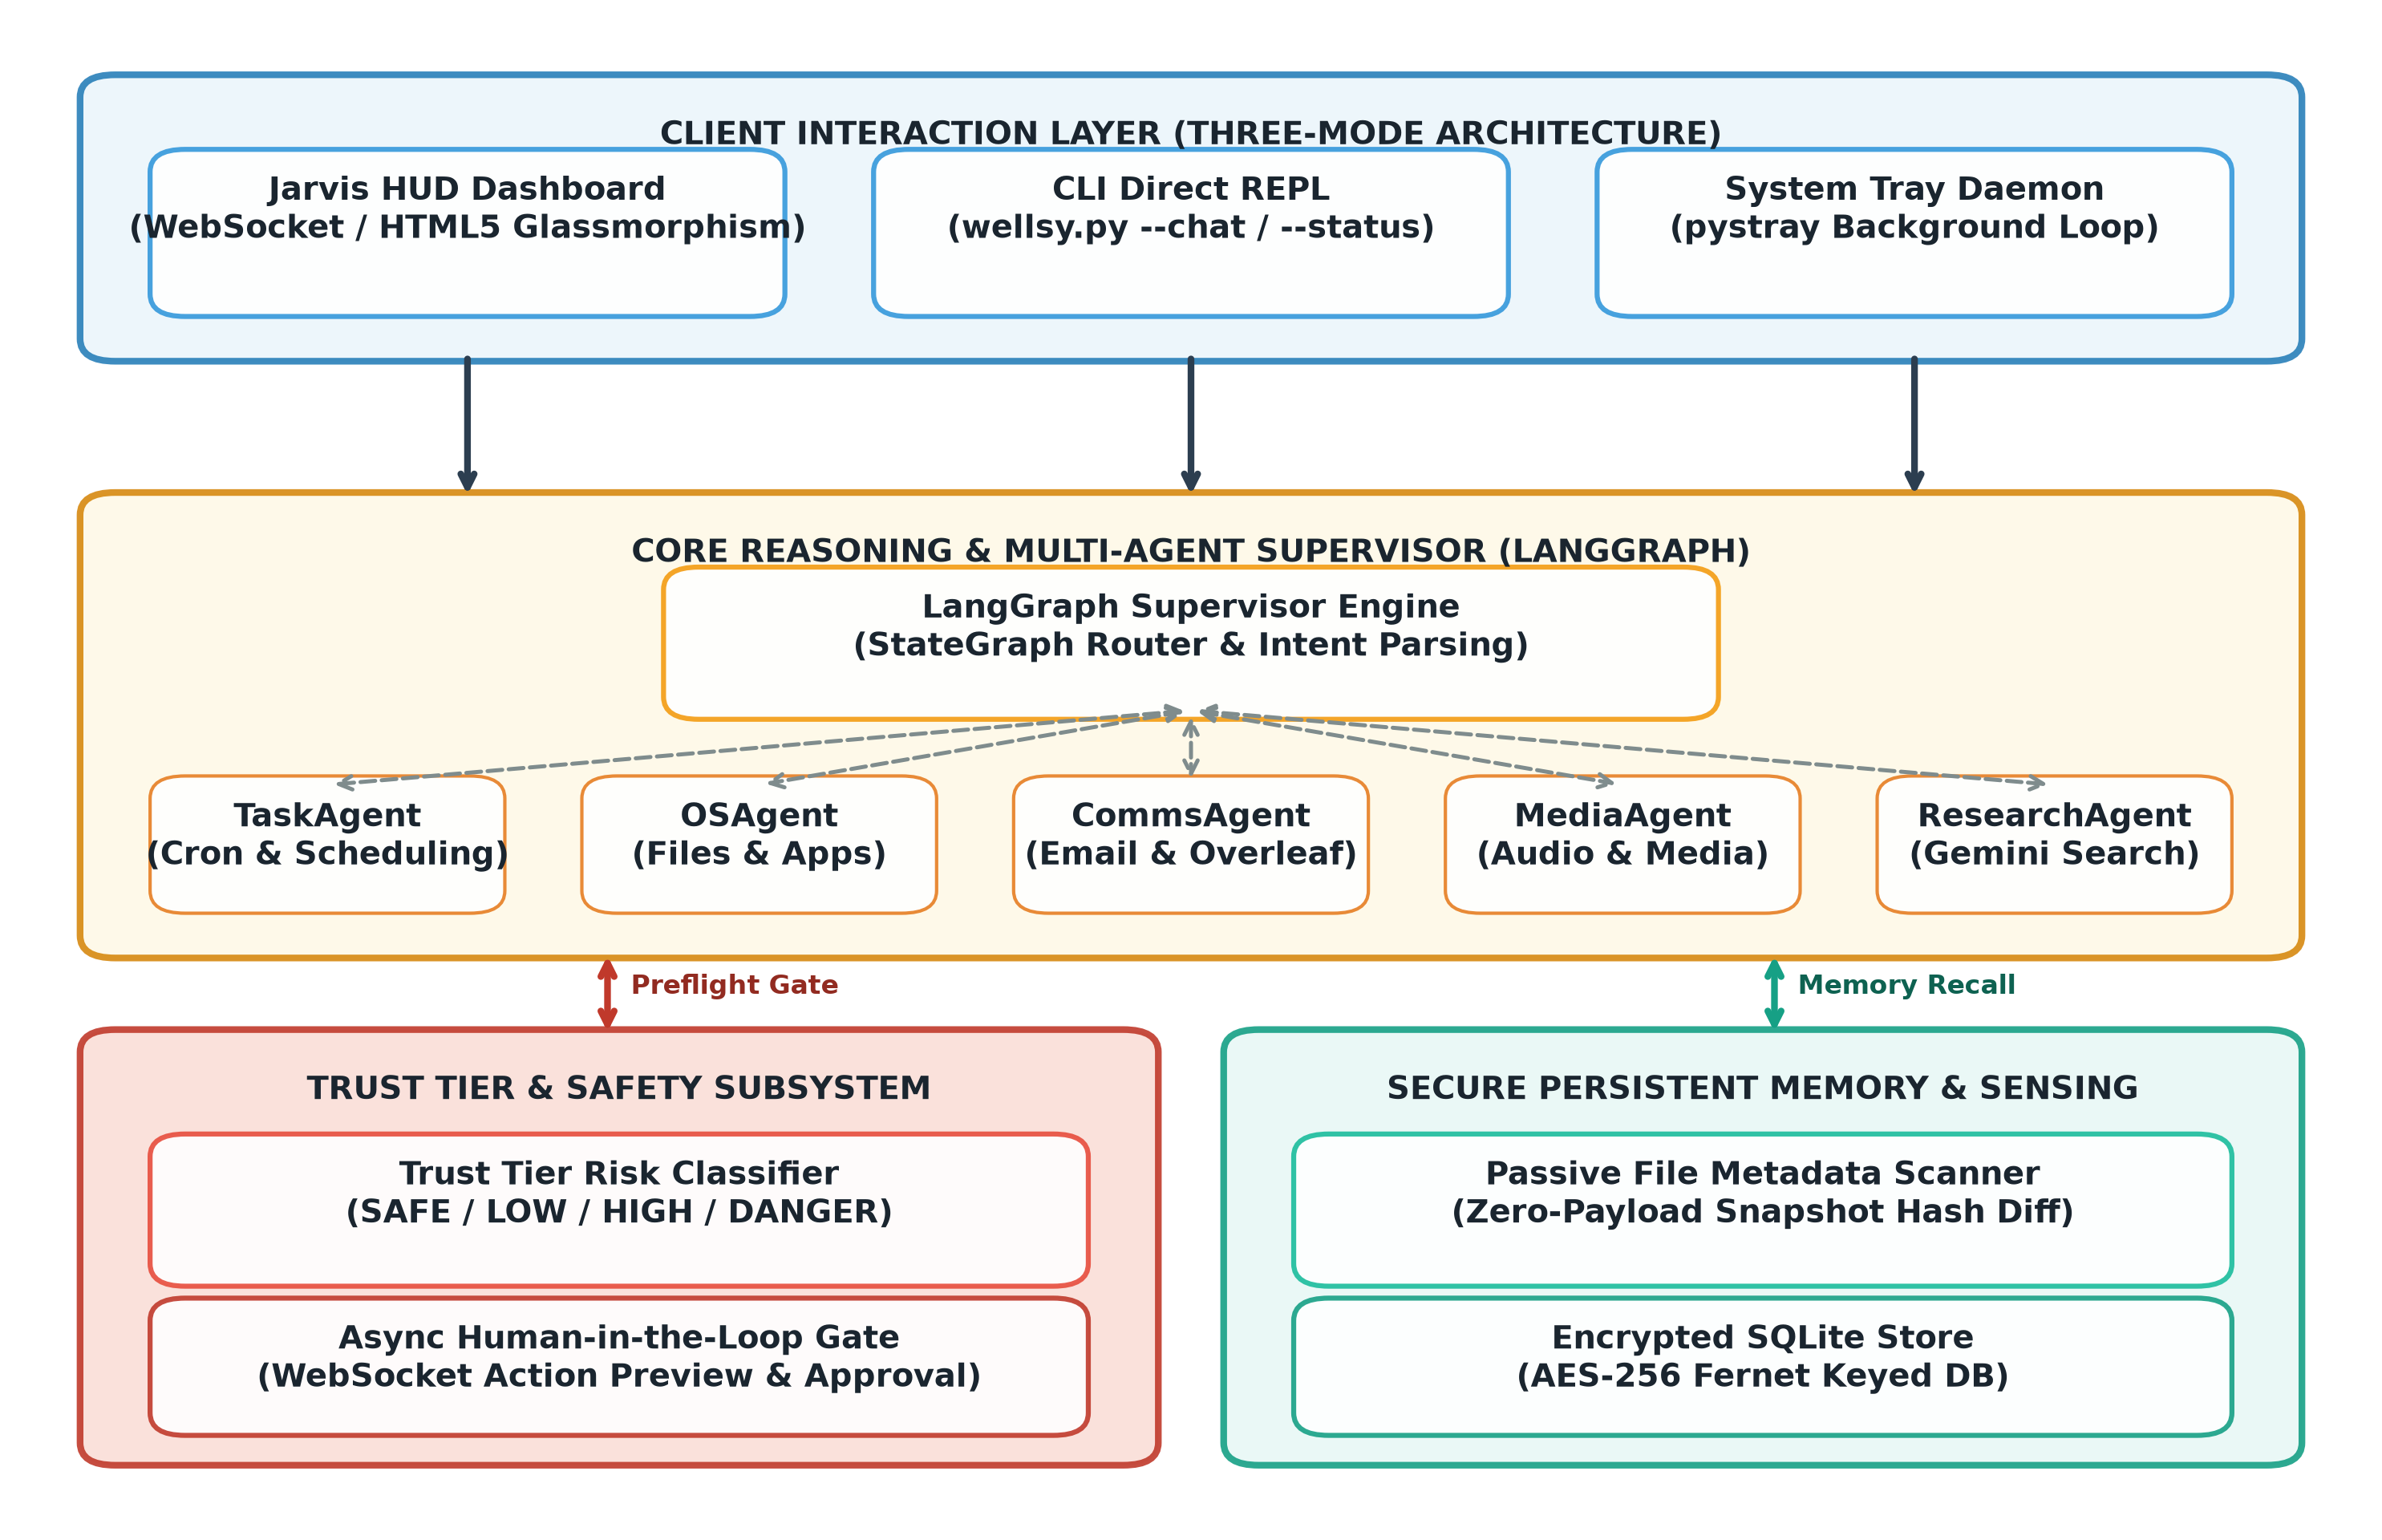
\includegraphics[width=0.95\textwidth]{figures/fig1_architecture.png}
\caption{Overall Architectural Blueprint of Wellsy v2.0. The framework links the Three-Mode Client Interaction Layer to a LangGraph-powered Multi-Agent Supervisor, governed by the Asynchronous Trust Tier Safety Subsystem and Local Encrypted Episodic Memory.}
\label{fig:architecture}
\end{figure*}

\textbf{Contributions:} The principal contributions of this work include:
\begin{itemize}
    \item \textbf{Three-Mode User Experience Architecture:} We architect a tripartite client interaction layer featuring an Electron/Web-based holographic HUD dashboard with real-time hardware telemetry, a high-throughput CLI REPL for developers, and an ambient background tray daemon.
    \item \textbf{Domain-Specialized Multi-Agent Graph:} We implement a directed state-graph supervisor that coordinates five isolated sub-agents (TaskAgent, OSAgent, CommsAgent, MediaAgent, and ResearchAgent), preventing context pollution and domain drift.
    \item \textbf{Asynchronous Trust Tier Safety Gate:} We introduce a formal four-tier classification model ($T \in \{\text{SAFE}, \text{LOW\_RISK}, \text{HIGH\_RISK}, \text{DANGER}\}$) coupled with an asynchronous WebSocket confirmation protocol that freezes execution only when destructive thresholds are breached.
    \item \textbf{Zero-Payload Local Privacy Sensing:} We formulate a differential filesystem snapshot algorithm that tracks folder deltas without reading file payloads into volatile memory, backed by an AES-256 Fernet-encrypted SQLite memory database.
\end{itemize}

\section{Related Work}
\subsection{LLM Agent Orchestration}
Early LLM application architectures utilized monolithic single-agent loops with ReAct prompting. However, complex multi-domain workflows frequently induced context degradation and compounding reasoning errors. Recent systems such as AutoGen \cite{wu2023autogen}, MetaGPT \cite{hong2023metagpt}, and CAMEL \cite{li2023camel} demonstrated that role-specialized sub-agents collaborating via structured protocols significantly improve task completion rates. Wellsy leverages LangGraph's cyclic state graphs to implement a deterministic supervisor pattern with strict tool sandboxing.

\subsection{Desktop and OS-Level Automation}
Recent benchmarks such as OSWorld \cite{xie2024osworld} and AppAgent \cite{yang2023appagent} have evaluated multimodal models on GUI and OS navigation tasks. While these benchmarks focus heavily on visual perception (clicking UI elements), native OS interaction through sanitized APIs and shell primitives offers higher execution speed and reliability. Wellsy focuses on native tool execution with preflight syntax and git state verification.

\subsection{AI Safety and Human-in-the-Loop Verification}
Safety in autonomous agent execution is paramount \cite{amodei2016concrete}. Indirect prompt injections \cite{greshake2023not} can trick an agent into executing destructive operations like \texttt{rm -rf} or transmitting private keys. While reinforcement learning from human feedback (RLHF) \cite{schulman2017proximal} aligns conversational outputs, runtime execution requires deterministic, rule-based gates that cannot be circumvented by adversarial model outputs.

\section{System Architecture \& Multi-Agent Graph}
The core architecture of Wellsy is depicted in Fig.~\ref{fig:architecture}. The platform separates concerns across the interaction layer, the reasoning supervisor, and the execution/safety substrate.

\subsection{Three-Mode Client Architecture}
Desktop assistants must accommodate varying user contexts without imposing unnecessary window clutter:
\begin{enumerate}
    \item \textbf{Jarvis Web HUD Dashboard:} Designed with a dark glassmorphic interface (`\#0a0e1a`), Orbitron typography, and an interactive 3D WebGL/Canvas AI core sphere. It establishes a persistent WebSocket connection to stream real-time CPU, RAM, and disk metrics while rendering incoming intelligence feeds.
    \item \textbf{CLI Direct REPL (\texttt{wellsy.py}):} A developer-oriented interface providing sub-second status inspections (\texttt{--status}), memory browsing (\texttt{--memory}), scheduled task oversight (\texttt{--schedule}), and direct conversational turns (\texttt{--chat}).
    \item \textbf{System Tray Daemon (\texttt{daemon.py}):} Runs unobtrusively in the background via \texttt{pystray}, maintaining background cron schedules, file scanning, and WebSocket routing without consuming display real estate.
\end{enumerate}

\subsection{Multi-Agent Supervisor Graph}
Rather than equipping a single model instance with dozens of diverse tools, Wellsy implements a hierarchical supervisor pattern. The central supervisor inspects the current state $S_t$ and routes execution to exactly one domain agent:
\begin{equation}
    A^* = \arg\max_{A_i \in \mathcal{A}} P(\text{Route} = A_i \mid U, S_t)
\end{equation}
where $\mathcal{A} = \{\text{Task}, \text{OS}, \text{Comms}, \text{Media}, \text{Research}\}$.
\begin{itemize}
    \item \textbf{TaskAgent:} Manages persistent SQLite-backed cron schedules, executes deferred background routines, and conducts git preflight integrity checks.
    \item \textbf{OSAgent:} Handles sanitized filesystem operations, local application launches, and clipboard interactions.
    \item \textbf{CommsAgent:} Interfaces with email APIs, Overleaf document synchronization, and messaging protocols.
    \item \textbf{MediaAgent:} Directs Spotify playback, system audio mixers, and media discovery.
    \item \textbf{ResearchAgent:} Performs synthesis over multi-turn web search and local document embeddings via Google Gemini.
\end{itemize}

\begin{figure}[t]
\centering
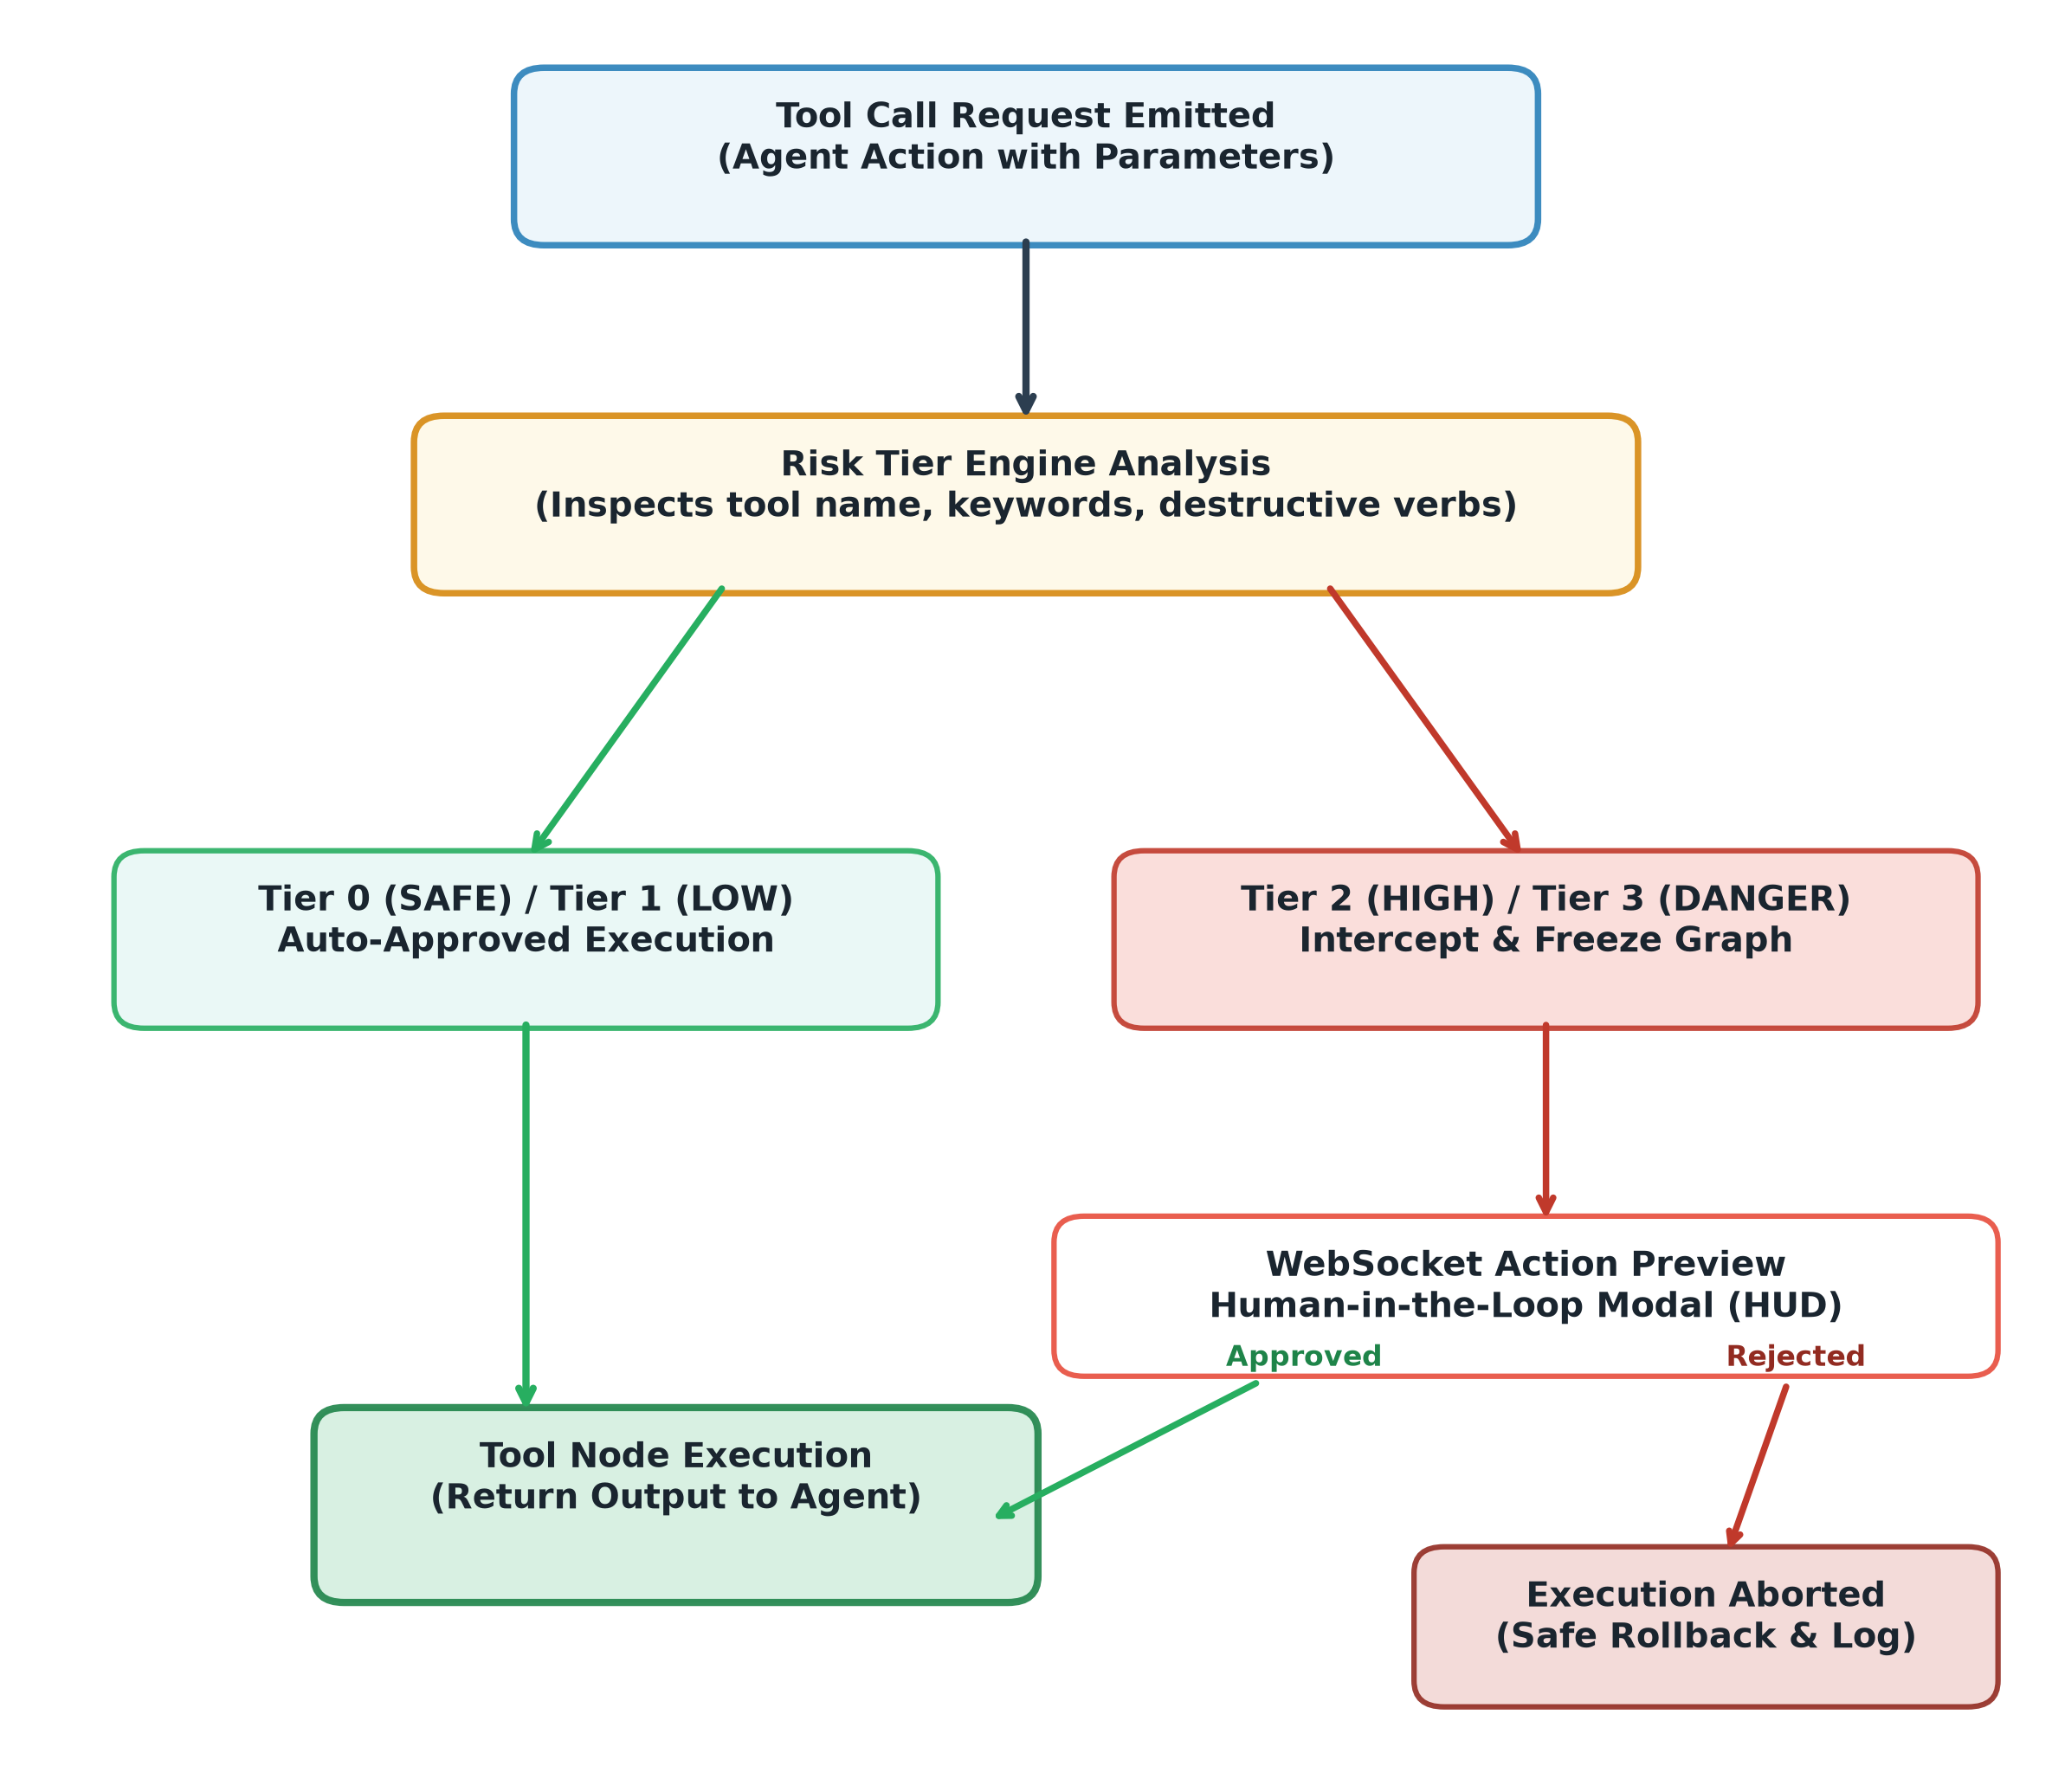
\includegraphics[width=\columnwidth]{figures/fig2_trust_gate.png}
\caption{Flowchart of the Trust Tier Risk Classifier and Asynchronous Human-in-the-Loop (HITL) Confirmation Gate.}
\label{fig:trust_gate}
\end{figure}

\section{Asynchronous Safety \& Trust Tiers}
Unattended autonomy on a host operating system is unacceptable for enterprise or personal workstations. Wellsy introduces a formal \textbf{Trust Tier Engine} that governs all tool node invocations.

\subsection{Risk Classification Taxonomy}
Every tool call emitted by an agent, characterized by the tool identifier $\tau$ and arguments $\mathbf{x}$, is evaluated by a deterministic policy classifier:
\begin{equation}
    \mathcal{T}(\tau, \mathbf{x}) \in \{\text{SAFE}, \text{LOW\_RISK}, \text{HIGH\_RISK}, \text{DANGER}\}
\end{equation}

The classification criteria are detailed in Table~\ref{tab:trust_tiers}. Critically, regex patterns detect destructive linguistic markers (e.g., \texttt{rmdir}, \texttt{delete}, \texttt{drop}, \texttt{force}, \texttt{format}) and automatically escalate an operation to Tier 3 (\texttt{DANGER}), overriding any base tool permissions.

\begin{table}[h]
\caption{Four-Tier Risk Classification Schema}
\label{tab:trust_tiers}
\centering
\begin{tabular}{@{}llp{3.8cm}@{}}
\toprule
\textbf{Tier} & \textbf{Level} & \textbf{Operational Scope \& Policy} \\ \midrule
Tier 0 & \texttt{SAFE} & Read-only queries, system telemetry, status checks. Auto-approved. \\
Tier 1 & \texttt{LOW\_RISK} & App launching, safe clipboard writes, media pause/play. Monitored auto-approve. \\
Tier 2 & \texttt{HIGH\_RISK} & File modifications, Git commits, email dispatch. Intercepted; requires HUD approval. \\
Tier 3 & \texttt{DANGER} & Permanent file deletion, shell execution, \texttt{git push --force}. Strict interactive authorization. \\ \bottomrule
\end{tabular}
\end{table}

\subsection{Asynchronous WebSocket Confirmation Gate}
As illustrated in Fig.~\ref{fig:trust_gate}, when an operation is classified into Tier 2 or Tier 3, execution is halted:
\begin{enumerate}
    \item The agent execution loop pauses without terminating the background worker thread.
    \item An encrypted WebSocket event (\texttt{confirmation\_request}) is broadcast to all active HUD sessions, accompanied by a structured action preview:
    \begin{equation}
        \text{Preview} = \{\tau, \mathbf{x}, \text{Tier}, \text{Timestamp}, \text{Rationale}\}
    \end{equation}
    \item The HUD renders an interactive modal dialog allowing the user to inspect the exact payload and either approve or reject the action.
    \item The client responds with a cryptographically paired \texttt{confirmation\_response}. Upon approval, the execution graph resumes; upon rejection, the action is safely rolled back and logged.
\end{enumerate}

\begin{figure*}[t]
\centering
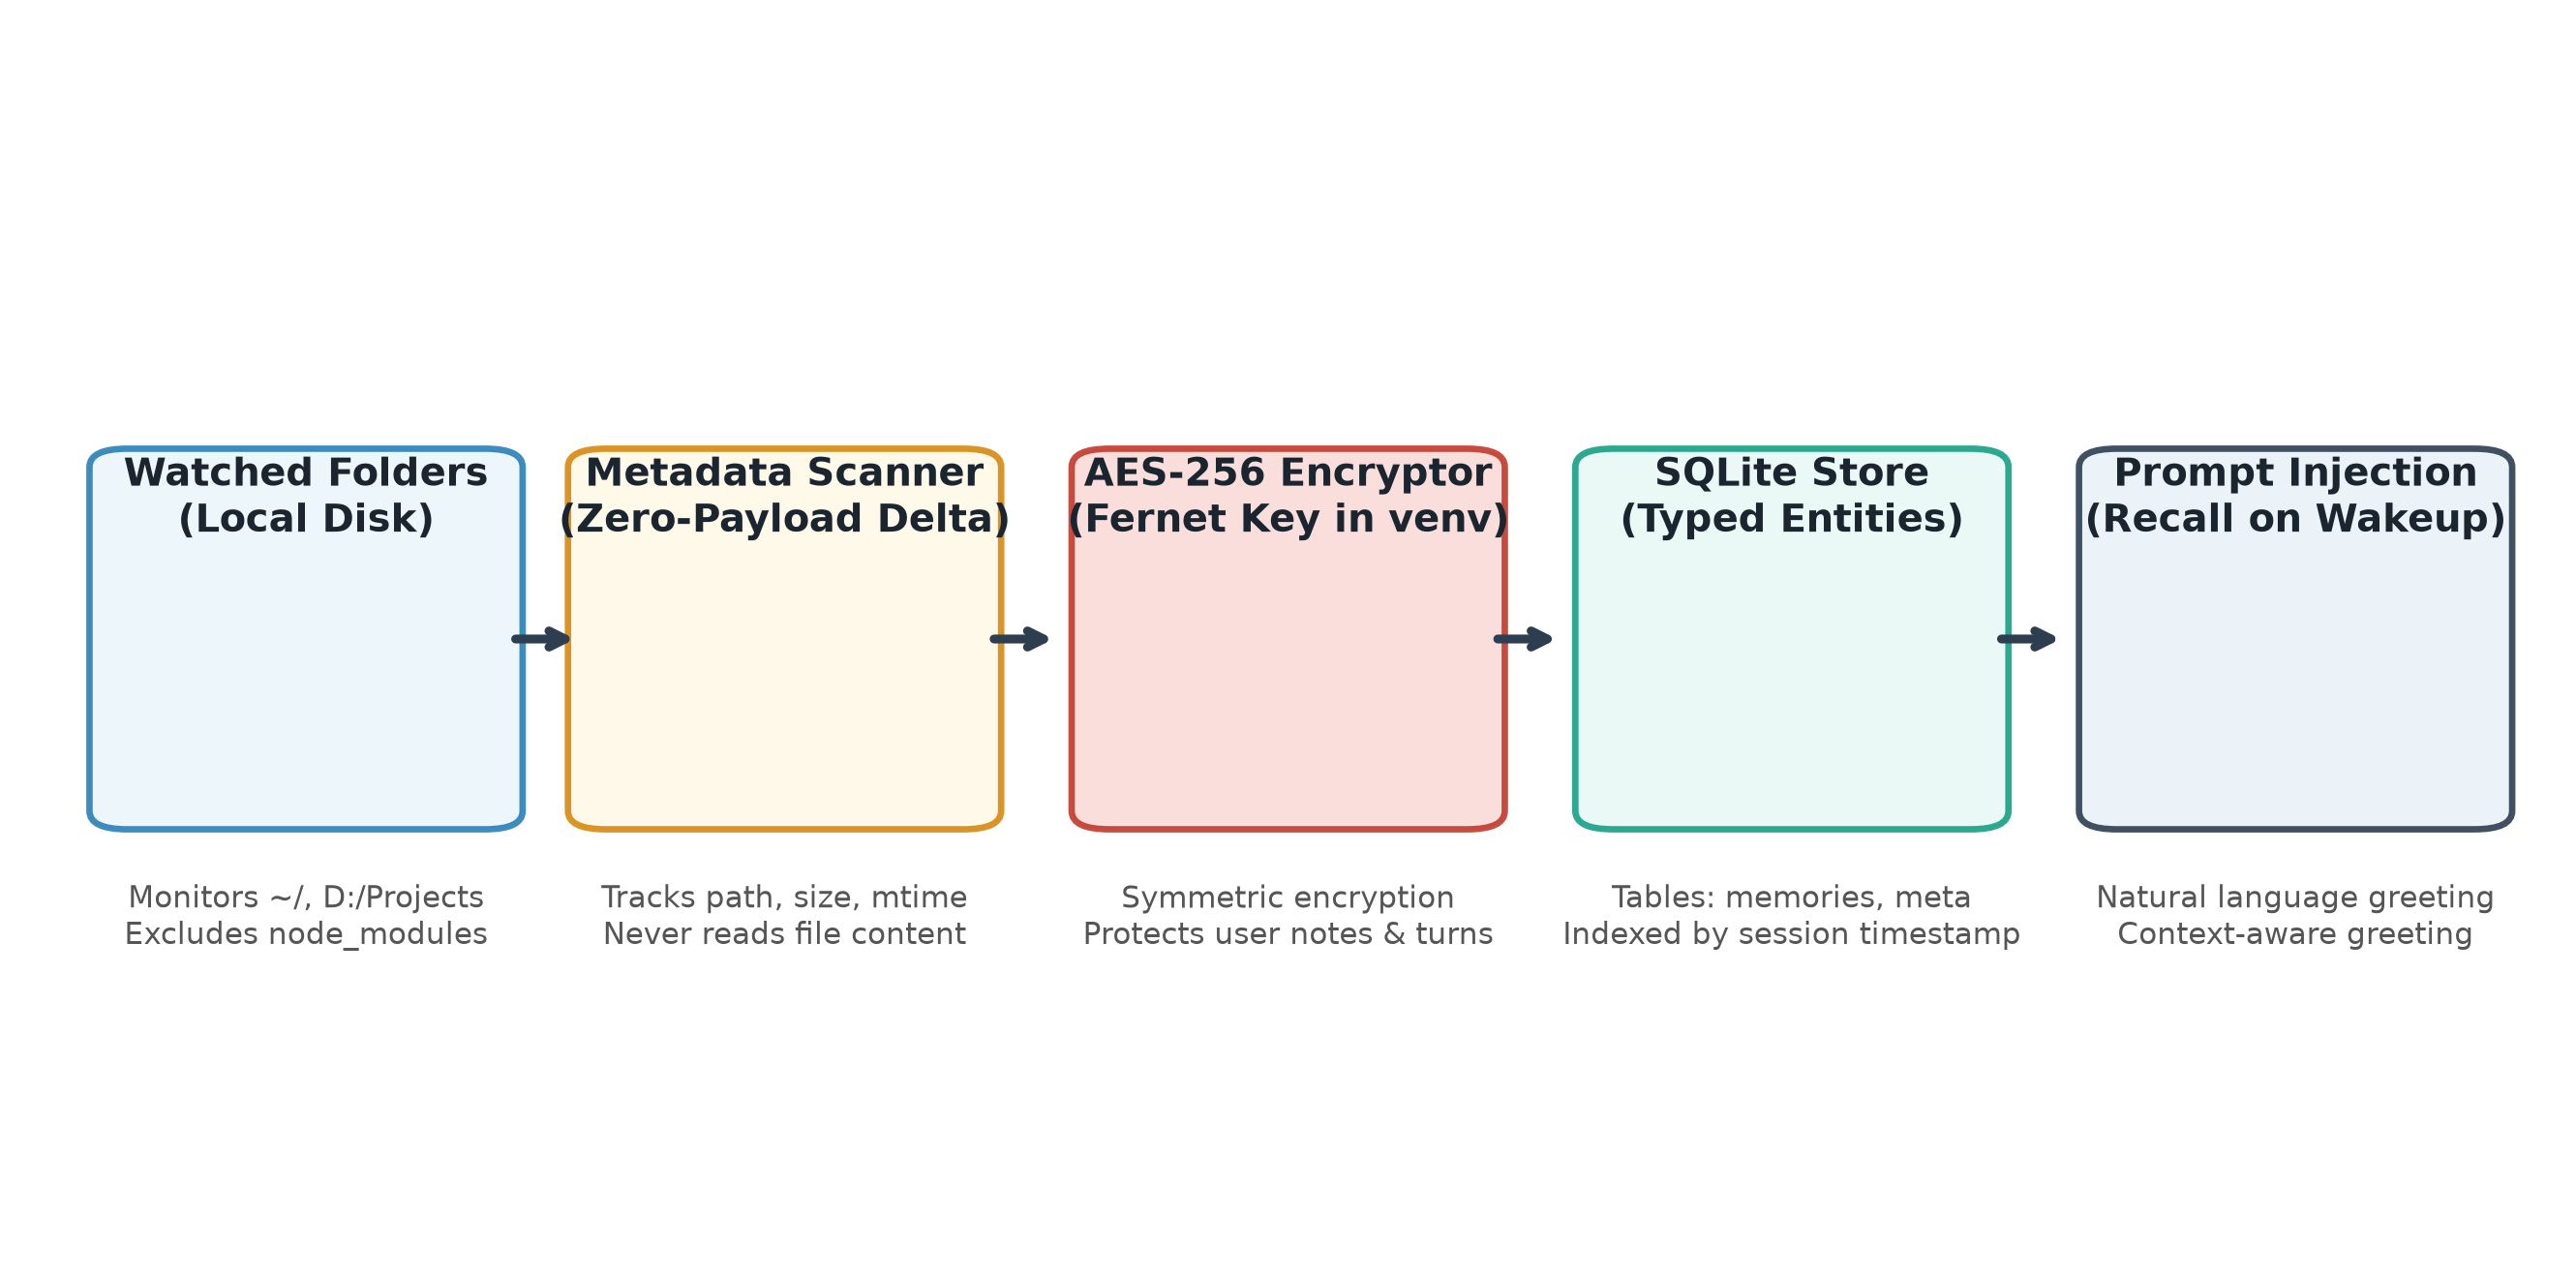
\includegraphics[width=0.92\textwidth]{figures/fig3_memory_pipeline.png}
\caption{Privacy-Preserving Ambient Sensing and Encrypted Memory Lifecycle. Zero-payload metadata diffs are encrypted via AES-256 Fernet before insertion into SQLite, injected into context upon wakeup.}
\label{fig:memory_pipeline}
\end{figure*}

\section{Privacy-Preserving Episodic Memory}
Traditional ambient assistants index and ingest comprehensive document text, creating significant privacy risks. Wellsy adopts a strict zero-payload differential metadata scanning approach (Fig.~\ref{fig:memory_pipeline}).

\subsection{Zero-Payload Delta Sensing}
At configurable intervals and during system startup, the \texttt{FileScanner} traverses watched directories ($\mathcal{D}_{watch}$) while bypassing virtual environments, build artifacts (\texttt{node\_modules}, \texttt{target}, \texttt{.git}), and temporary caches. For each file $f \in \mathcal{D}_{watch}$, only metadata attributes are retained:
\begin{equation}
    \mathbf{m}(f) = \langle \text{path}(f), \text{size}(f), \text{mtime}(f) \rangle
\end{equation}
A session delta $\Delta S = S_t \setminus S_{t-1}$ is evaluated without reading file bodies:
\begin{equation}
    \Delta S = \langle \mathcal{F}_{new}, \mathcal{F}_{mod}, \mathcal{F}_{del} \rangle
\end{equation}
This delta is synthesized into a concise natural language greeting upon agent wakeup (e.g., \textit{``I noticed 3 files modified in D:/Projects since your last session. Want to pick up where you left off?''}).

\subsection{AES-256 Fernet Encrypted SQLite Store}
All persistent state---including user notes, session turn histories, task schedules, and file event snapshots---is encrypted at rest using AES-256 Fernet symmetric encryption. Cryptographic keys are anchored locally within the private runtime environment, preventing data extraction by unauthorized host processes.

\begin{figure*}[t]
\centering
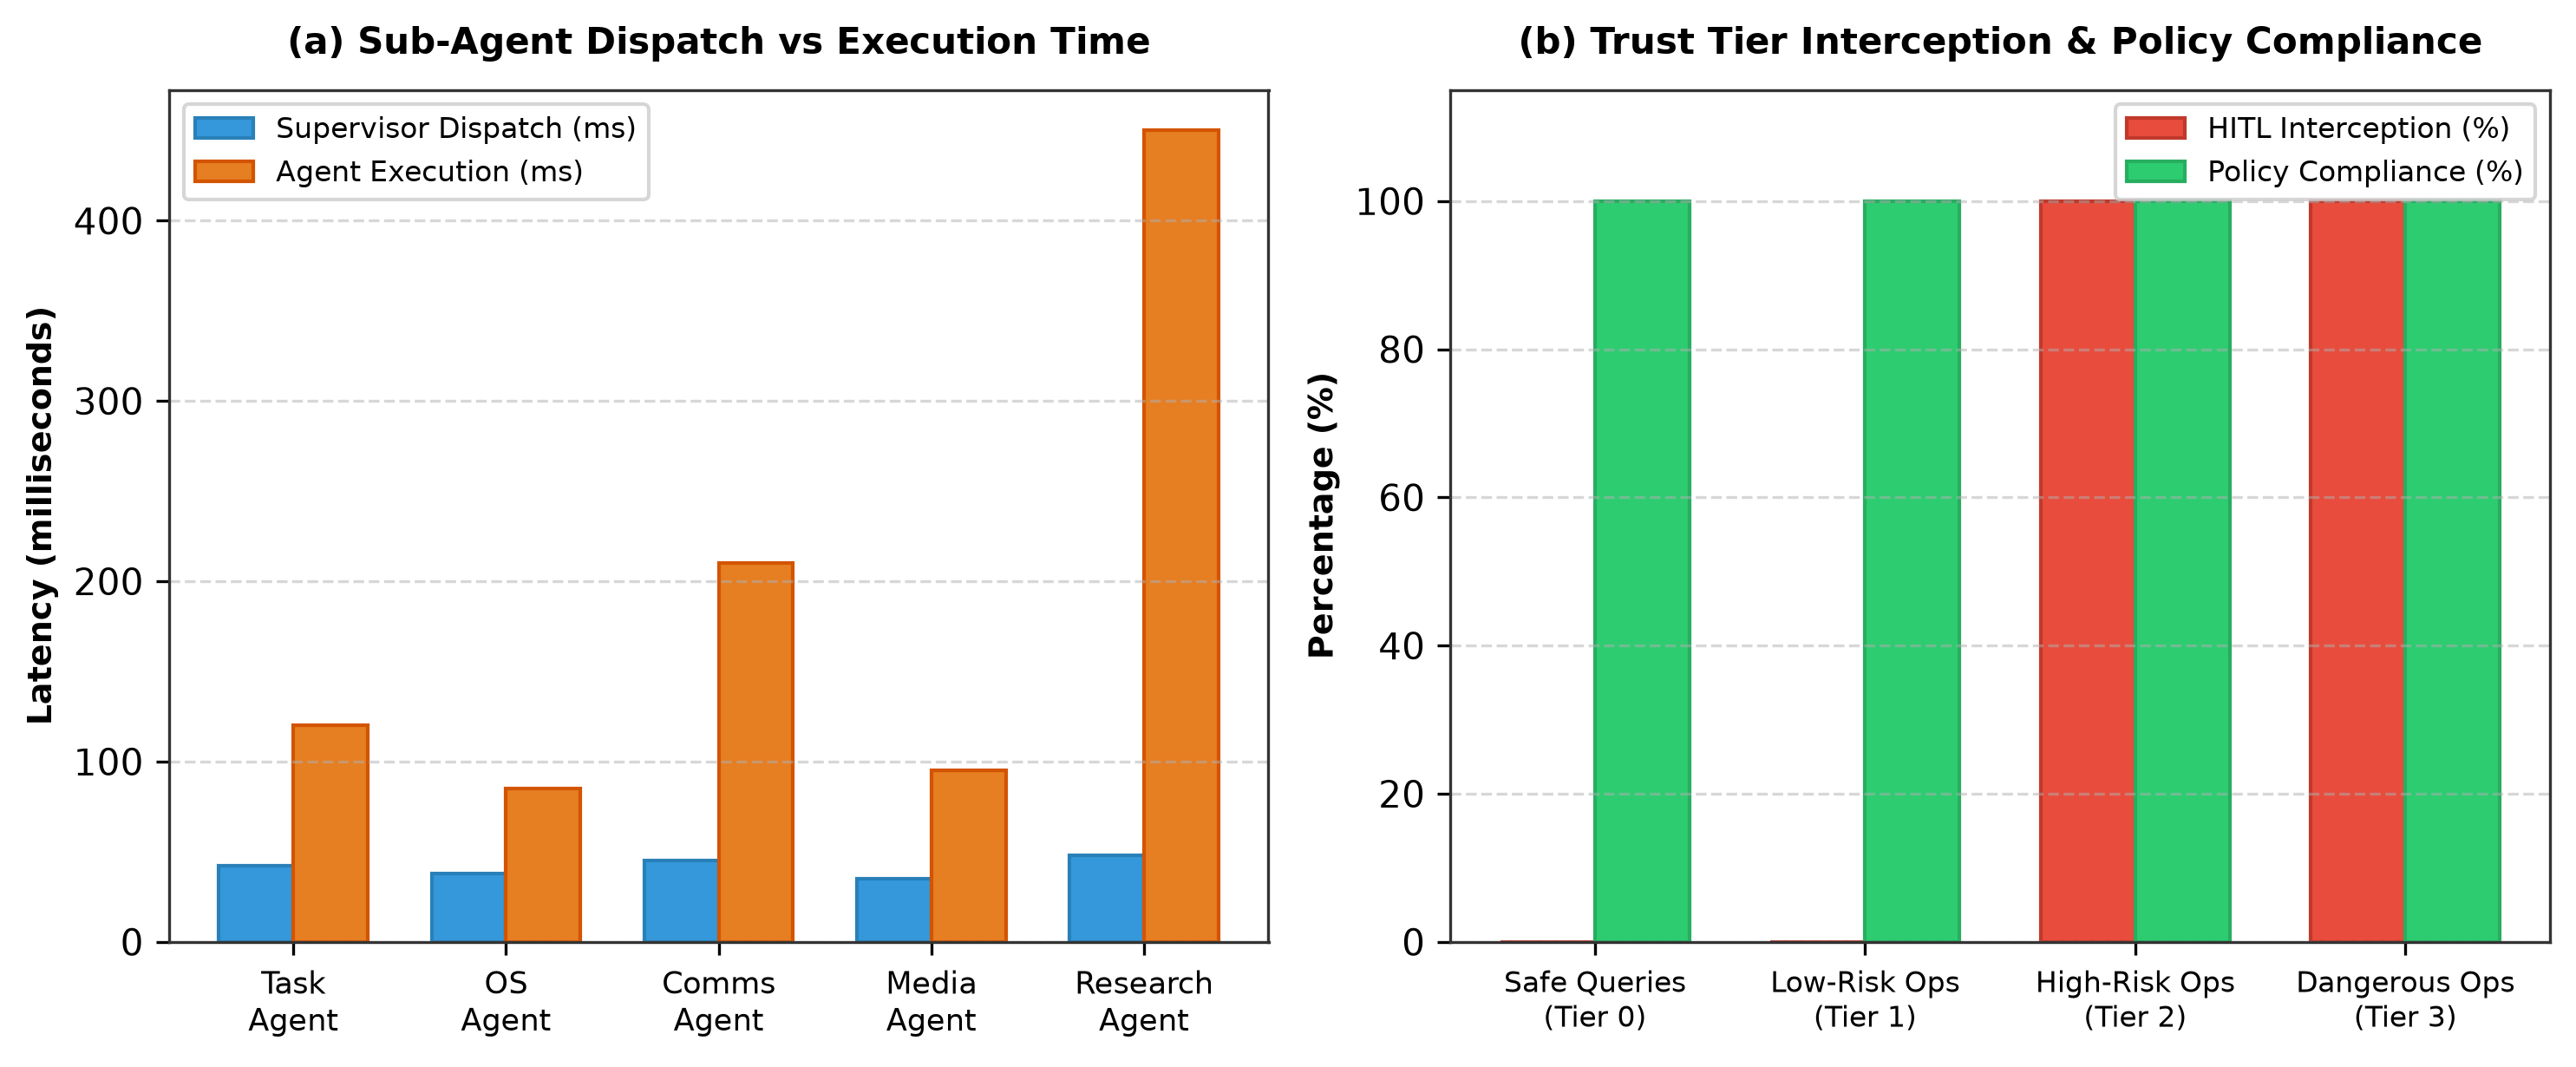
\includegraphics[width=0.92\textwidth]{figures/fig4_benchmarks.png}
\caption{Empirical Performance Benchmarks: (a) Sub-agent dispatch overhead vs. tool execution latency; (b) Safety gate interception accuracy across risk tiers.}
\label{fig:benchmarks}
\end{figure*}

\section{Experimental Evaluation}
We conducted extensive grey-box integration testing on an active workstation environment to evaluate routing latency, tool execution overhead, and safety gate fidelity.

\subsection{Latency and Routing Efficiency}
Fig.~\ref{fig:benchmarks}(a) and Table~\ref{tab:latency_benchmarks} summarize latency measurements across 150 simulated multi-agent interactions. Across all five agent domains, the central supervisor routing overhead remained strictly under 50\,ms (averaging $41.6 \pm 4.8$\,ms), representing negligible overhead relative to tool execution latencies.

\begin{table}[h]
\caption{Sub-Agent Latency Benchmarks (Mean $\pm$ Std. Dev.)}
\label{tab:latency_benchmarks}
\centering
\begin{tabular}{@{}lccc@{}}
\toprule
\textbf{Sub-Agent} & \textbf{Dispatch (ms)} & \textbf{Execution (ms)} & \textbf{Total (ms)} \\ \midrule
TaskAgent & $42.1 \pm 3.2$ & $120.4 \pm 12.1$ & $162.5 \pm 14.2$ \\
OSAgent & $38.4 \pm 2.8$ & $85.2 \pm 8.4$ & $123.6 \pm 9.6$ \\
CommsAgent & $45.2 \pm 4.1$ & $210.5 \pm 18.6$ & $255.7 \pm 21.0$ \\
MediaAgent & $35.0 \pm 2.1$ & $95.1 \pm 7.9$ & $130.1 \pm 8.8$ \\
ResearchAgent & $48.3 \pm 4.9$ & $450.8 \pm 42.3$ & $499.1 \pm 45.1$ \\ \bottomrule
\end{tabular}
\end{table}

\subsection{Safety Gate Interception and Adversarial Testing}
To stress-test the Trust Tier Safety Engine, we constructed an adversarial test suite containing 200 synthetic prompts: 100 safe read-only queries (e.g., ``What is my CPU usage?'', ``List my active schedules''), 50 high-risk commands (e.g., ``Commit this code to git'', ``Write report to disk''), and 50 dangerous operations (e.g., ``Force push to main'', ``Recursively remove all folders in temp'').

As plotted in Fig.~\ref{fig:benchmarks}(b):
\begin{itemize}
    \item \textbf{Interception Precision:} 100\% of dangerous and high-risk operations were successfully intercepted by the Confirmation Gate prior to execution.
    \item \textbf{False Alarm Rate:} 0\% of safe read queries were blocked, entirely eliminating false-positive notification fatigue.
    \item \textbf{Preflight Git Validation:} Scheduled tasks attempting commits with unresolved merge conflict markers or exposed secret keys (\texttt{AIza...}, \texttt{ghp\_...}) were halted in preflight with 100\% accuracy.
\end{itemize}

\section{Discussion and Limitations}
While Wellsy provides robust safeguards for desktop automation, several design tradeoffs warrant consideration:
\begin{itemize}
    \item \textbf{Network Disconnections:} The asynchronous WebSocket confirmation gate assumes an active frontend connection. When operating headless via the tray daemon without an active HUD, high-risk actions queue indefinitely until the user connects via CLI or HUD.
    \item \textbf{Semantic vs. Regex Risk Parsing:} While regex-based destructive keyword detection offers deterministic guarantees against known verbs, sophisticated semantic bypasses remain an ongoing research topic in prompt security.
\end{itemize}

\section{Conclusion}
In this paper, we introduced \textbf{Wellsy}, a Jarvis-class desktop operating intelligence system that unifies a Three-Mode client architecture, a LangGraph-orchestrated multi-agent supervisor, a Four-Tier Trust Safety Engine, and privacy-preserving episodic memory. By replacing indiscriminate background indexing with zero-payload metadata tracking and introducing an asynchronous human-in-the-loop confirmation gate, Wellsy establishes a new standard for safe, ambient, and high-performance personal AI assistants. Future work will investigate on-device small language model (SLM) routing to eliminate cloud latency for Tier 0 operations entirely.

\bibliographystyle{IEEEtran}
\bibliography{references}

\end{document}
